\documentclass[aspectratio=169]{beamer}
\usepackage[T1]{fontenc}
\usepackage[utf8]{inputenc}
\usepackage{tikz}
\usepackage{tabularx}
\usepackage[font=scriptsize]{caption}
\captionsetup[figure]{labelformat=empty}

\usetikzlibrary{tikzmark,shapes,arrows,backgrounds,fit,positioning}
\newcolumntype{C}{>{\centering\arraybackslash}X}
\newcolumntype{R}{>{\raggedleft\arraybackslash}X}

\addtobeamertemplate{navigation symbols}{}
{
	\insertframenumber{}
}

\beamertemplatenavigationsymbolsempty
\setbeamercolor{section in foot}{fg=white, bg=blue}
\setbeamercolor{subsection in foot}{fg=black, bg=white}
\setbeamerfont{footline}{size=\fontsize{6}{6}\selectfont}

\setbeamertemplate{footline}
{
  \leavevmode
  \hbox
  {
    \begin{beamercolorbox}
      [wd=.5\paperwidth,ht=2.5ex,dp=1.125ex,leftskip=.3cm,rightskip=.3cm]{subsection in foot}
    \end{beamercolorbox}
    
    \begin{beamercolorbox}
      [wd=.5\paperwidth,ht=2.5ex,dp=1.125ex,leftskip=.3cm,rightskip=.3cm plus1fil]{subsection in foot}
      \hfill
      \insertframenumber
      %\insertframenumber\,/\,\inserttotalframenumber
    \end{beamercolorbox}
  }
}



\title{UUB Charge and Peak histograms}
\author{
  Mauricio Su\'arez Dur\'an and Ioana~C.~Mari\c{s}
}
\institute{IIHE-ULB}

\titlegraphic{
  \begin{figure}[h]
    \centering
   %
\includegraphics[width=5cm]{ulbLogo2.png}
    \hspace*{8.cm}
    
\includegraphics[width=5.5cm]{iihe.jpeg}
  \end{figure}
}

\begin{document}
\begin{frame}
  \titlepage
\end{frame}


\begin{frame}
	\frametitle{UUB Charge and Peak histograms}
	\begin{itemize}
		\item Station studied: 863 1222 1219 1211 1740 1743 1221 1223 1217 1747 1741 1745 1818 1851 1729 1735 1746 1819 1791
		\item Data from CDAS.
		\item {\underline {Software CDAS, pre-production version.}}
	\end{itemize}
	\centering
	\includegraphics[width=.45\textwidth]{mapStations.pdf}
\end{frame}


\begin{frame}
  \begin{figure}
    \centering
    \begin{tabularx}{\textwidth}{CC}
      \begin{tabular}{l}
        Let's assume a muon pulse as \\
        exponential function: \\
        $P(t) = P_{\mathrm{max}}\exp(-t/\tau)$. \\ \\
        
        So, the peak takes a value of $P_{\mathrm{max}}$, and \\
        the integral (A) takes $P_{\mathrm{max}}\tau$. \\ \\

        This means an AoP of $\tau$. \\ \\

        In a digitalized scenario, the $P(t)$ \\
        takes values each $\Delta t$, which \\
        means that the $P_{\mathrm{max}}$ will be a value \\
        between $P(ts)$ and $P(ts + \Delta t)$, where $ts$ \\
        is the time at which the signal starting. \\ \\
        Let's say that peak is at $ts$, then \\
        $P(ts) = P_{\mathrm{max}}\exp(-ts/\tau)$. \\
      \end{tabular}
      &
      \begin{tabular}{l}
        For the integral: \\
        $A = \Delta t \sum_{n=1}^{n=\infty} 
        P_{\mathrm{max}}\exp{-\frac{ts + n\Delta t}{\tau}}$ \\

        $A = P_{\mathrm{max}} \exp^{-ts/\tau} 
        \frac{\Delta t}{1 - e^{-\Delta t/\tau}}$ \\ \\

        Therefore, we expected an AoP of \\
        $\mathrm{AoP} = \frac{\Delta t}{1 - e^{-\Delta t/\tau}}$. \\ \\

        If $\Delta t$ goes to zero, so
        $\mathrm{AoP} = \tau$ 
      \end{tabular}
    \end{tabularx}
  \end{figure}
\end{frame}

\begin{frame}
  For UB, AoP takes: \\
  $\left( \mathrm{AoP}\right)^{\mathrm{UB}} 
  = \frac{25\,\mathrm{ns}}{1 - e^{-25/\tau}}$\, \\
  and for UUB, \\
  $\left( \mathrm{AoP}\right)^{\mathrm{UUB}}
  = \frac{8.33\,\mathrm{ns}}{1 - e^{-8.33/\tau}}$ \\

  So, 
  $\frac{ \left( \mathrm{AoP}\right)^{\mathrm{UB}} }
  { \left(\mathrm{AoP}\right)^{\mathrm{UUB}} }
  = \frac{25\,\mathrm{ns} \left( 1 - e^{-8.33/\tau} \right)}
  {8.33\,\mathrm{ns} \left( 1 - e^{-25/\tau} \right)}$ \\

  $\frac{ \left( \mathrm{AoP}\right)^{\mathrm{UB}} }
  { \left(\mathrm{AoP}\right)^{\mathrm{UUB}} }
  = 3 \frac{\left( 1 - e^{-8.33/\tau} \right)}{\left( 1 - e^{-25/\tau} \right)} $\\

  Assuming a $\tau=50$\,ns: \\
  
  $\frac{ \left( \mathrm{AoP}\right)^{\mathrm{UB}} }
  { \left(\mathrm{AoP}\right)^{\mathrm{UUB}} }
  = 3 \frac{0.15}{0.39} = 1.17$ \\

  $\left( \mathrm{AoP}\right)^{\mathrm{UB}} = 1.17 \left(\mathrm{AoP}\right)^{\mathrm{UUB}} $




\end{frame}
%\begin{frame}
%  \frametitle{Checking for UUB Peak histograms}
%  \begin{figure}
%    \centering
%    \begin{tabularx}{\textwidth}{CC}
%      \begin{tabular}{l}
%        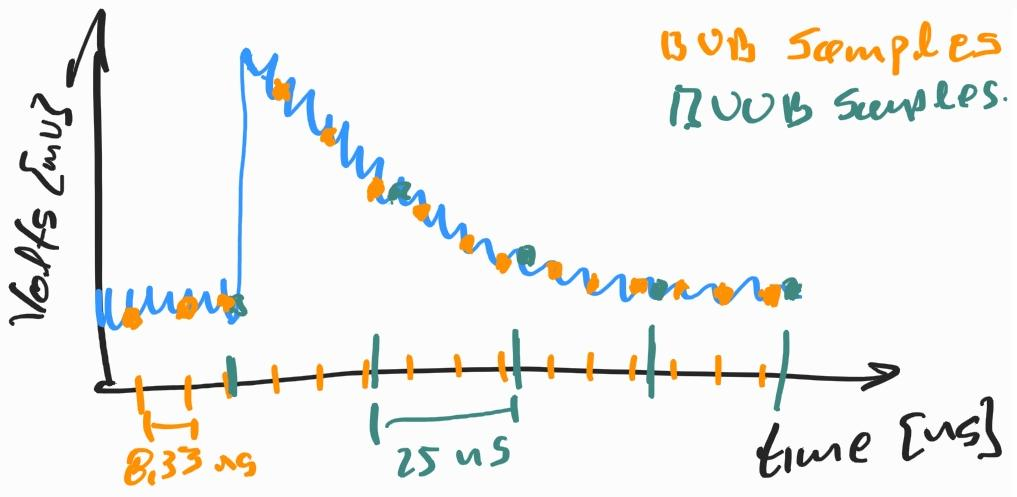
\includegraphics[width=.4\textwidth]{pulseSamples.jpg}
%      \end{tabular}
%      \vspace{0.2cm}
%
%      \begin{tabular}{l}
%        At first approx., we expect a bigger\\
%        UUB VEM-Peak than UB VEM-Peak.\\ \\
%        So, $\frac{1 (\mathrm{VEM}_\mathrm{pk}^{\mathrm{UUB}})} {1 (\mathrm{VEM}_\mathrm{pk}^{\mathrm{UB}})}$
%        $ = \frac{N_\mathrm{pk}^{\mathrm{UUB}}*(0.49\,\mathrm{mV}/8.33\,\mathrm{ns})}
%        {N_\mathrm{pk}^{\mathrm{UB}}*(1.95\,\mathrm{mV}/25\,\mathrm{ns})}$\\ \\
%
%        Where $0.49$\,mV $= 2$\,V$/2^{12}$ and\\ 
%        $1.95$\,mV $= 2$\,V$/2^{10}$, and $N_\mathrm{pk}^{i}$ is the counts\\
%        in FADC, respectively.
%      \end{tabular}
%      &
%      \begin{tabular}{l}
%        This means, if this pulse resprents a VEM,\\
%        we will have a ratio of
%      \end{tabular}
%      \vspace{0.2cm}
%
%      \begin{tabular}{l}
%        $\frac{1 (\mathrm{VEM}_\mathrm{pk}^{\mathrm{UUB}})} {1 (\mathrm{VEM}_\mathrm{pk}^{\mathrm{UB}})} 
%        = \left(\frac{3}{4}\right)
%        \left( \frac{N_\mathrm{pk}^{\mathrm{UUB}}} {N_\mathrm{pk}^{\mathrm{UB}}}\right)$\\ \\
%        So, we expect that $ N_\mathrm{pk}^{\mathrm{UUB}}/N_\mathrm{pk}^{\mathrm{UB}}>4/3$. \\ \\
%        Caveat: this has sense if the pulse \\
%        is the same (HV more or less the same).\\ \\
%        Let's check for Station 863.
%      \end{tabular}
%    \end{tabularx}
%  \end{figure}
%\end{frame}
%
%% ============================
%% *** Checking for St. 863 ***
%
%\begin{frame}
%	\frametitle{Checking ratio $\frac{N_\mathrm{pk}^{\mathrm{UUB}}} {N_\mathrm{pk}^{\mathrm{UB}}}$ for St. 863}
%  \begin{figure}
%  \centering
%    \begin{tabularx}{\textwidth}{C}
%      \includegraphics[width=.65\textwidth]{../plots/uubPeaktimeHbSt863PMTs.png}
%      \\
%      Removing values for november, we have as average:
%      \\
%      \begin{tabular}{l}
%        For {\bf PMT1}: $n_\mathrm{pk}(\mathrm{FADC})_\mathrm{UUB} = 137.16$, 
%        and $n_\mathrm{pk}(\mathrm{FADC})_\mathrm{UB} = 36.76$. {\bf Ratio:} $3.73$
%      \end{tabular}
%      \begin{tabular}{l}
%        For {\bf PMT2}: $n_\mathrm{pk}(\mathrm{FADC})_\mathrm{UUB} = 164.95$, 
%        and $n_\mathrm{pk}(\mathrm{FADC})_\mathrm{UB} = 26.56$. {\bf Ratio:} $6.21$
%      \end{tabular}
%      \begin{tabular}{l}
%        For {\bf PMT3}: $n_\mathrm{pk}(\mathrm{FADC})_\mathrm{UUB} = 142.79$, 
%        and $n_\mathrm{pk}(\mathrm{FADC})_\mathrm{UB} = 43.04$. {\bf Ratio:} $3.32$
%      \end{tabular}
%    \end{tabularx}
%  \end{figure}
%\end{frame}
%
%
%\begin{frame}
%  \frametitle{Checking for St. 863's HV}
%  Data from /pbs/throng/pauger/DATA/Raid/monit/ and readed with TSDMonCal.h
%  \centering
%  \vspace{0.5cm}
%
%  \includegraphics[width=.8\textwidth]{../plots/uubHVSt863.png}
%\end{frame}
%
%\begin{frame}
%  \frametitle{Checking for St. 863's HV}
%  From http://mon.auger.uni-wuppertal.de/pro/SD/LS/Monitoring.php?LSId=863
%  \begin{figure}
%    \centering
%    \begin{tabularx}{\textwidth}{CC}
%      \includegraphics[width=.5\textwidth]{../plots/hvPMT1uub.png}
%      &
%      \includegraphics[width=.5\textwidth]{../plots/hvPMT2uub.png}
%      \\
%      \includegraphics[width=.5\textwidth]{../plots/hvPMT3uub.png}
%      &
%      \includegraphics[width=.5\textwidth]{../plots/hvPMT1ub.png}
%    \end{tabularx}
%  \end{figure}
%\end{frame}
%
%\begin{frame}
%  \frametitle{Checking for St. 863's HV}
%  From http://mon.auger.uni-wuppertal.de/pro/SD/LS/Monitoring.php?LSId=863
%  \centering
%  \vspace{0.5cm}
%
%  \includegraphics[width=1.\textwidth]{../plots/hvPMT1ub.png}
%\end{frame}
%
%
%\begin{frame}
%  \frametitle{A/P}
%  \begin{figure}
%    \centering
%    \begin{tabularx}{\textwidth}{CC}
%      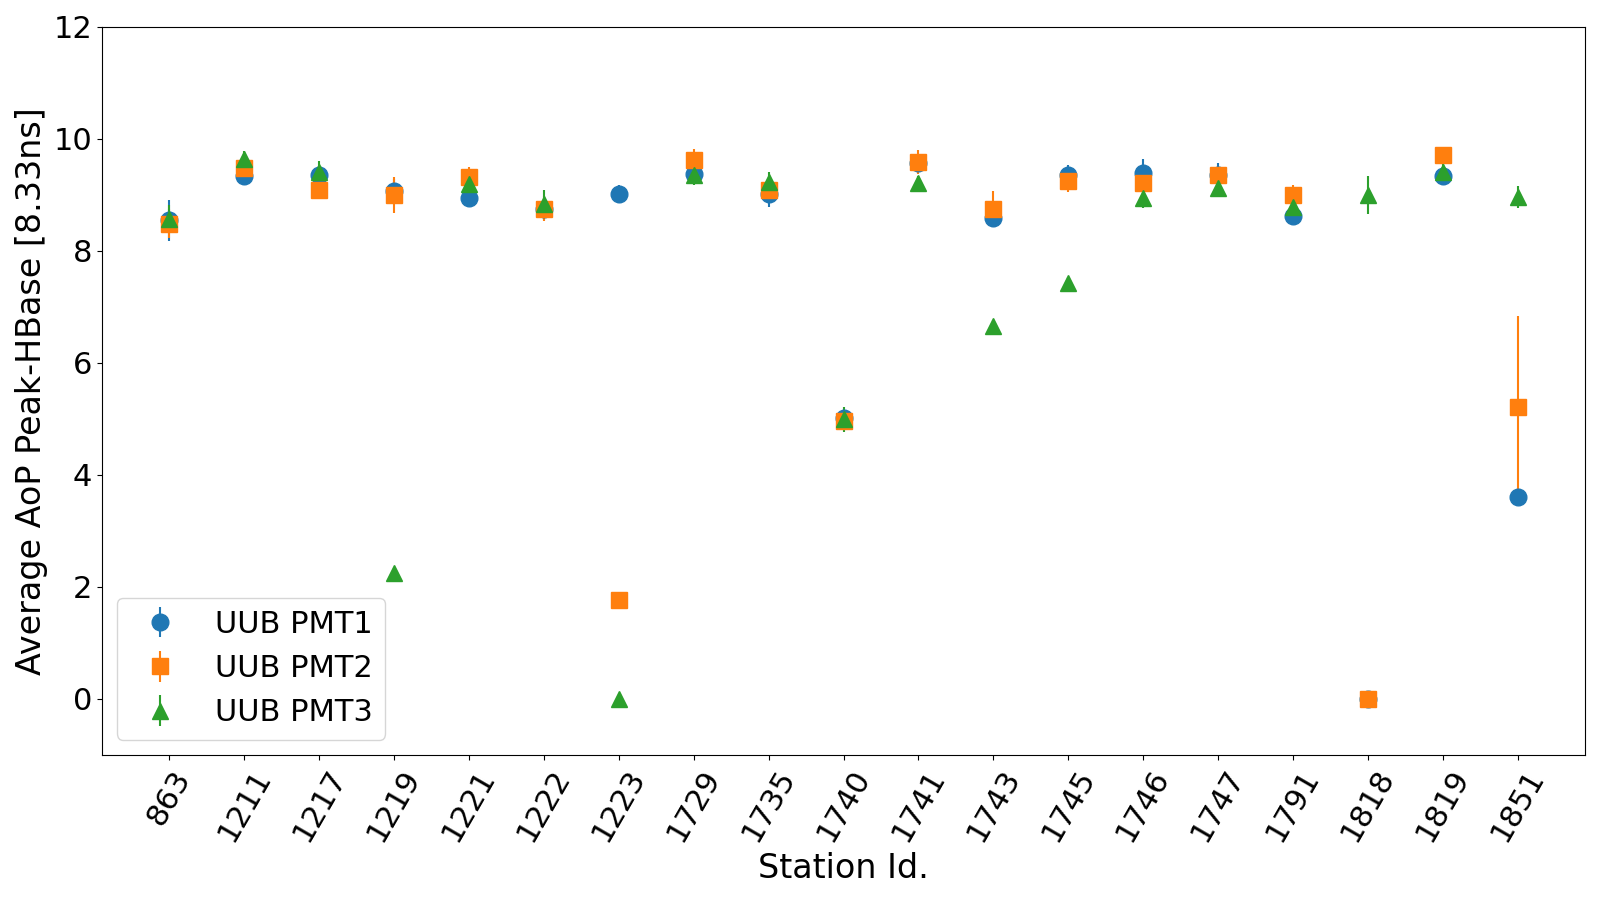
\includegraphics[width=.45\textwidth]{../plots/uubAoPHbasePMTs.png}
%      &
%      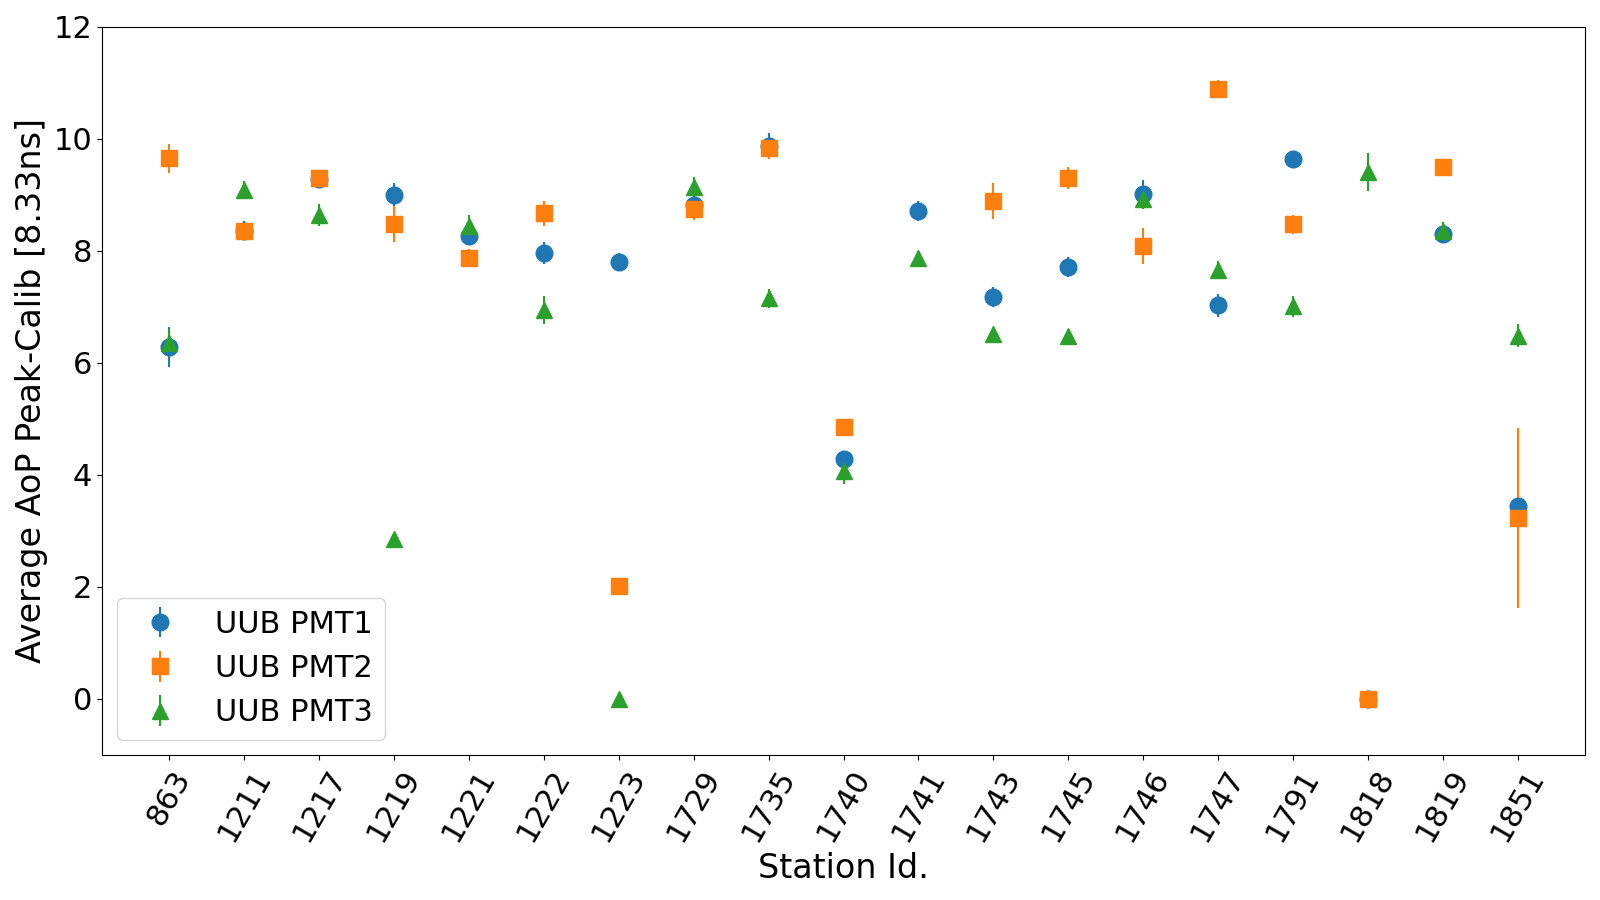
\includegraphics[width=.45\textwidth]{../plots/uubAoPCalibPMTs.png}
%      \\
%      \includegraphics[width=.45\textwidth]{../plots/ubAoPHbasePMTs.png}
%      &
%      \includegraphics[width=.45\textwidth]{../plots/ubAoPCalibPMTs.png}
%    \end{tabularx}
%  \end{figure}
%  \centering
%  
%\end{frame}
%
%
%\begin{frame}
%  \frametitle{A/P Relative difference for Peak corrections}
%  \begin{figure}
%    PMTs with AoP lower than $4$\,ns for UUB and $2$\,ns for UB are not considered here.
%    \centering
%    \begin{tabularx}{\textwidth}{CC}
%      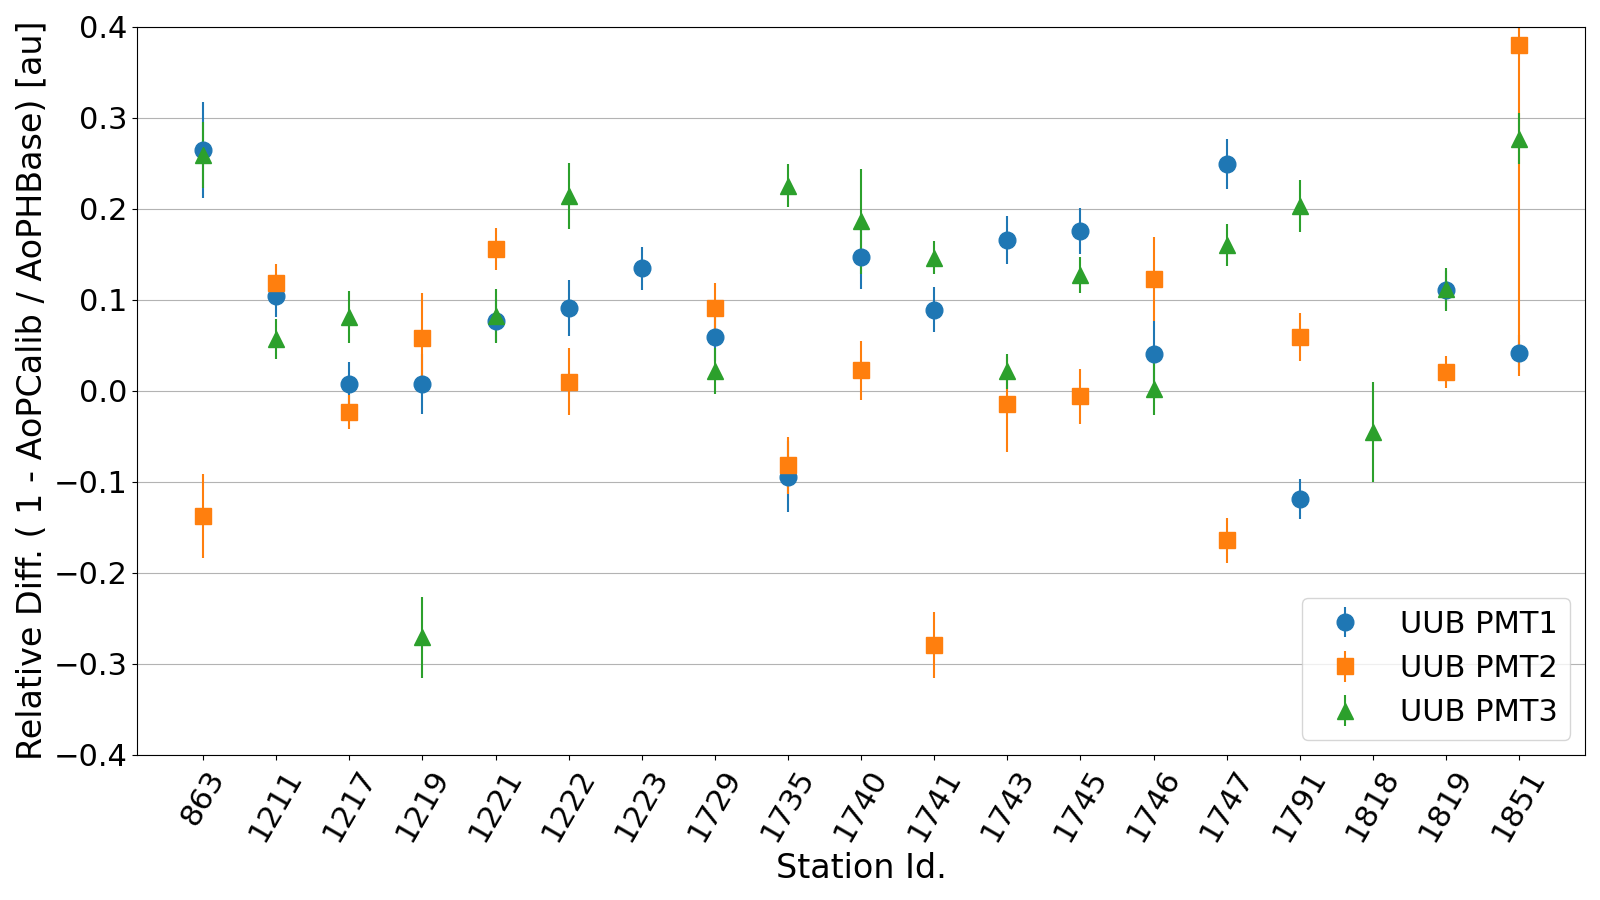
\includegraphics[width=.43\textwidth]{../plots/uubAoPDiffCaHbPMTs.png}
%      &
%      \includegraphics[width=.43\textwidth]{../plots/ubAoPDiffCaHbPMTs.png}
%      \\
%      \includegraphics[width=.43\textwidth]{../plots/aopHbaseUubUbPMTs.png}
%      &
%      \includegraphics[width=.43\textwidth]{../plots/aoCalibUubUbPMTs.png}
%    \end{tabularx}
%  \end{figure}
%\end{frame}
%
%
%\begin{frame}
%	\frametitle{Peak and Charge over time}
%  \begin{figure}
%  \centering
%    \begin{tabularx}{\textwidth}{CC}
%      \includegraphics[width=.5\textwidth]{../plots/uubPeaktimeHbSt863PMTs.png}
%      &
%      \includegraphics[width=.5\textwidth]{../plots/uububChargetimeHbSt863PMTs.png}
%    \end{tabularx}
%  \end{figure}
%\end{frame}
%
%\begin{frame}
%	\frametitle{Peak and Charge over time}
%  \begin{figure}
%  \centering
%    \begin{tabularx}{\textwidth}{CC}
%      \includegraphics[width=.5\textwidth]{../plots/uubPeaktimeHbSt1740PMTs.png}
%      &
%      \includegraphics[width=.5\textwidth]{../plots/uububChargetimeHbSt1740PMTs.png}
%    \end{tabularx}
%  \end{figure}
%\end{frame}
%
%
%\begin{frame}
%	\frametitle{Peak and Charge over time}
%  \begin{figure}
%  \centering
%    \begin{tabularx}{\textwidth}{CC}
%      \includegraphics[width=.5\textwidth]{../plots/uubPeaktimeHbSt1219PMTs.png}
%      &
%      \includegraphics[width=.5\textwidth]{../plots/uububChargetimeHbSt1219PMTs.png}
%    \end{tabularx}
%  \end{figure}
%\end{frame}
%
%
%\begin{frame}
%  \frametitle{How well is the fit method works? }
%  {\bf Events-Fitting / Events-total }
%	\begin{figure}
%		\centering
%    \begin{tabularx}{\textwidth}{CC}
%      \begin{tabular}{l}
%        \includegraphics[width=.44\textwidth]{../plots/uubGoodFitEvtnPk.png}
%      \end{tabular}
%      &
%			\begin{tabular}{l}
%				\includegraphics[width=.44\textwidth]{../plots/ubGoodFitEvtnPk.png}
%			\end{tabular}
%			\\
%			\begin{tabular}{l}
%				\includegraphics[width=.44\textwidth]{../plots/uubGoodFitEvtnChPMT.png}
%			\end{tabular} 
%      &
%      \begin{tabular}{l}
%        \includegraphics[width=.44\textwidth]{../plots/ubGoodFitEvtnChPMT.png}
%      \end{tabular}
%		\end{tabularx}
%	\end{figure}
%\end{frame}



\end{document}
